\chapter{Analysis and Design}
\section{Introduction}
\par
This chapter provides an explanation of our project design in the following sections: analysis of
the existing system, user requirement analysis, and system design. First is analysis of the existing
system, this section evaluates the current systems and applications available in the market,
identifying their features, limitations, and areas for improvement along with the PlanADay
application. Second,the user requirement analysis section that explains the features of the project.
Third, the system design user diagrams consist of a context diagram, data flow diagram, activity
diagram, use case diagram, system sequence diagram, flow chart, and key-valued database
diagram.

\section{Analysis of the existing system}
Currently, several applications are available in the market that assist users in planning trips, such
as Google Maps, Strippl, Gethergo, and ChatGPT. These platforms offer various features,
including route navigation, attraction suggestions, and itinerary planning. However, they differ in
their ability to cater to specific user needs.
\par
For instance, most existing applications, like Google Maps and Strippl, are well-suited for users
who already know where they want to go, as they provide efficient routing paths and
location-based directions. Similarly, Gethergo offers recommendations based on user-defined
interests but requires users to input detailed preferences or destinations. On the other hand,
PlanADay offers catering to users who may not have a clear idea of where they want to go. The
application generates personalized, one-day trip plans based on broad user interests, preferences,
and current location, offering a complete itinerary without requiring extensive input or prior
knowledge of specific destinations. The comparison table below summarizes the key features of
each application.

\newpage
\begin{table}[]
    \begin{tabular}{|l|c|c|c|c|c|}
    \hline
    \rowcolor[HTML]{C0C0C0} 
    Feature                                                                                       & \multicolumn{1}{l|}{\cellcolor[HTML]{C0C0C0}Strippl} & \multicolumn{1}{l|}{\cellcolor[HTML]{C0C0C0}gethergo} & \multicolumn{1}{l|}{\cellcolor[HTML]{C0C0C0}Google Map} & \multicolumn{1}{l|}{\cellcolor[HTML]{C0C0C0}ChatGPT} & \multicolumn{1}{l|}{\cellcolor[HTML]{C0C0C0}PlanADay} \\ \hline
    Require less input                                                                            & \checkmark                                           & -                                                     & \checkmark                                              & -                                                    & \checkmark                                            \\ \hline
    \begin{tabular}[c]{@{}l@{}}Suggest plan base on user\\ interests and preferences\end{tabular} & -                                                    & \checkmark                                            & -                                                       & \checkmark                                           & \checkmark                                            \\ \hline
    Suggest route based on location                                                               & \checkmark                                           & \checkmark                                            & \checkmark                                              & -                                                    & \checkmark                                            \\ \hline
    Real-time place Details                                                                       & -                                                    & \checkmark                                            & \checkmark                                              & -                                                    & \checkmark                                            \\ \hline
    Provide routing path                                                                          & \checkmark                                           & \checkmark                                            & \checkmark                                              & -                                                    & \checkmark                                            \\ \hline
    Generate/ Regenerate plan                                                                     & -                                                    & -                                                     & -                                                       & \checkmark                                           & \checkmark                                            \\ \hline
    Save related plan from others                                                                 & \checkmark                                           & \checkmark                                            & \checkmark                                              &                                                      & \checkmark                                            \\ \hline
    Overview Detail                                                                               & -                                                    & \checkmark                                            & \checkmark                                              & -                                                    & \checkmark                                            \\ \hline
    \end{tabular}
    \caption{Table of the feature comparisons}
    \label{tab:my-table}
\end{table}
\par
The PlanADay application aims to address these limitations by offering a more personalized and
flexible experience. It not only generates customized one-day trip plans based on user interests
but also allows users to adjust itineraries, share plans with others in the community, and
bookmark suggestions for future use. By bridging these gaps, PlanADay seeks to provide a more
user-focused and collaborative solution compared to existing systems.

\section{User requirement analysis}
The user requirement analysis aims to identify the expectations, preferences, and functional
needs of users who seek efficient and personalized one-day trip planning. Below is a breakdown
of the key user requirements that they might found:
\begin{enumerate}
    \item Users do not get the satisfied plan from the user’s input.
    \begin{itemize}
        \item Customization plan: Users can edit the plan which is delete the place, add more
        places, and reorder the place on their own again to make the most appropriate
        plan for the user.
    \end{itemize}
    \item Users want to change their preferences.
    \begin{itemize}
        \item Preference setting: Users can reselect their preferences all the time in application.
    \end{itemize}
    \item Users do not have any specific input.
    \begin{itemize}
        \item Suggestion plan: The application provides the plan that are generated from other
        users, so the user can use other’s plan to travel.
    \end{itemize}
\end{enumerate}
\newpage
\section{System Design}
\subsection{Use case diagram}
\begin{figure}[!h]
    \centering
    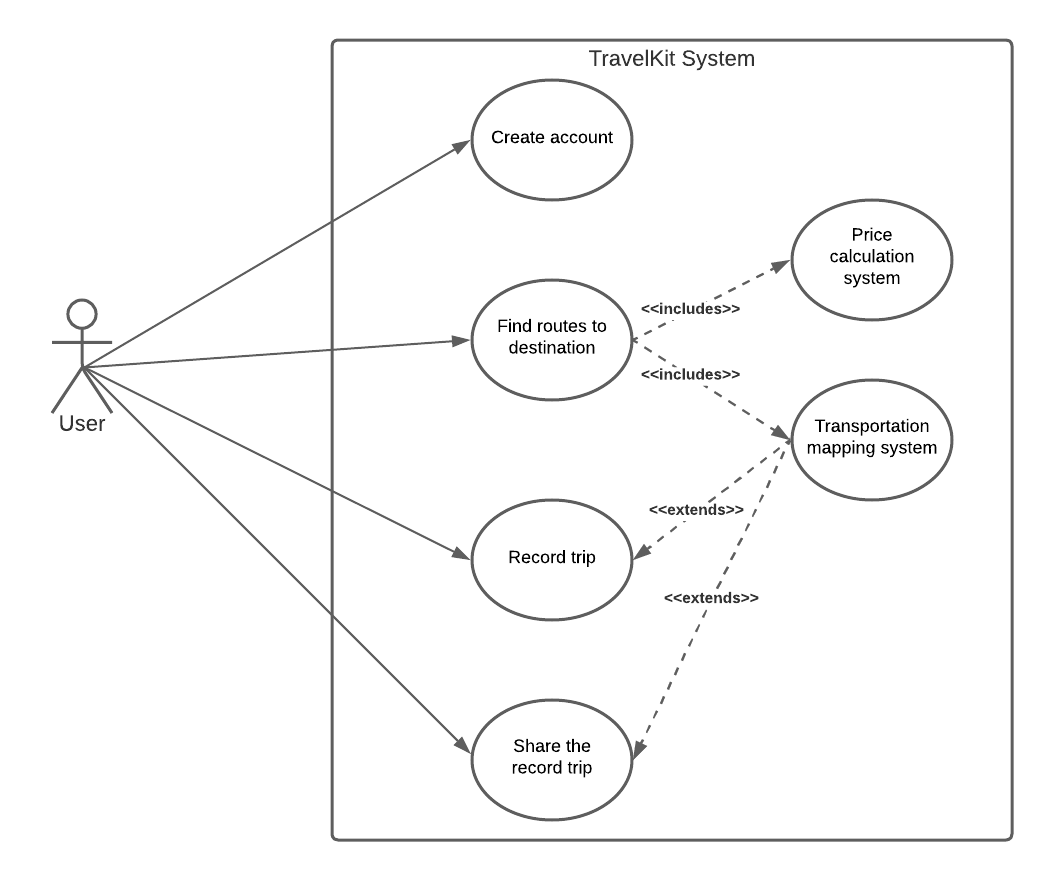
\includegraphics[width=0.7\linewidth]{chapter3/use-case-diagram.png}
    \caption{Use case diagram}
    \label{fig:Use case diagram}
\end{figure}
\par
The Actors who are in the PlanAday System. The user must create the account to authenticate in
the system. After the user input all field forms to create a plan, including the plan name, place
type, location, date and time and amount of places, The system will generate the plan and
display it to the user. if the user is not satisfied they can customize the plan by rearrange,
regenerate. The suggestion plans will show the public plans that mean each plan is shared by
other users. and filter the plan by user preferences.
\newpage
\subsection{Context diagram}
\begin{figure}[!h]
    \centering
    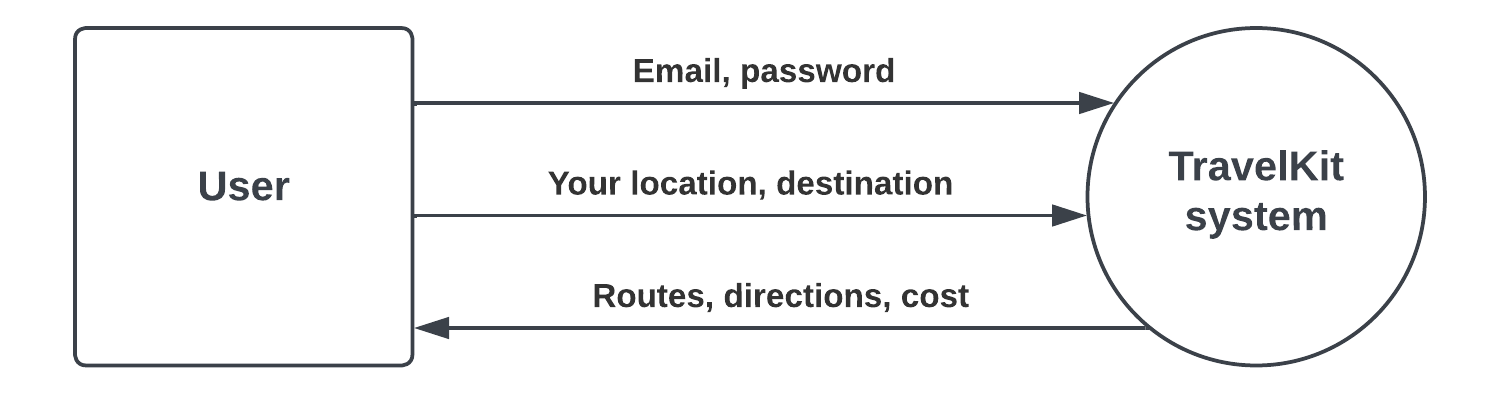
\includegraphics[width=1\linewidth]{chapter3/context-diagram.png}
    \caption{Context diagram}
    \label{fig:Context diagram}
\end{figure}
\par
The context diagram shows the overall of PlanADay System that requires the username,
password that need to be used in authentication service, place categories, location, date and time,
amount of places that need to be used in generating the plan. Then the system will provide a plan
that matches with input that includes details.

\newpage
\subsection{Activity Diagram}
Authentication process
\begin{figure}[!h]
    \centering
    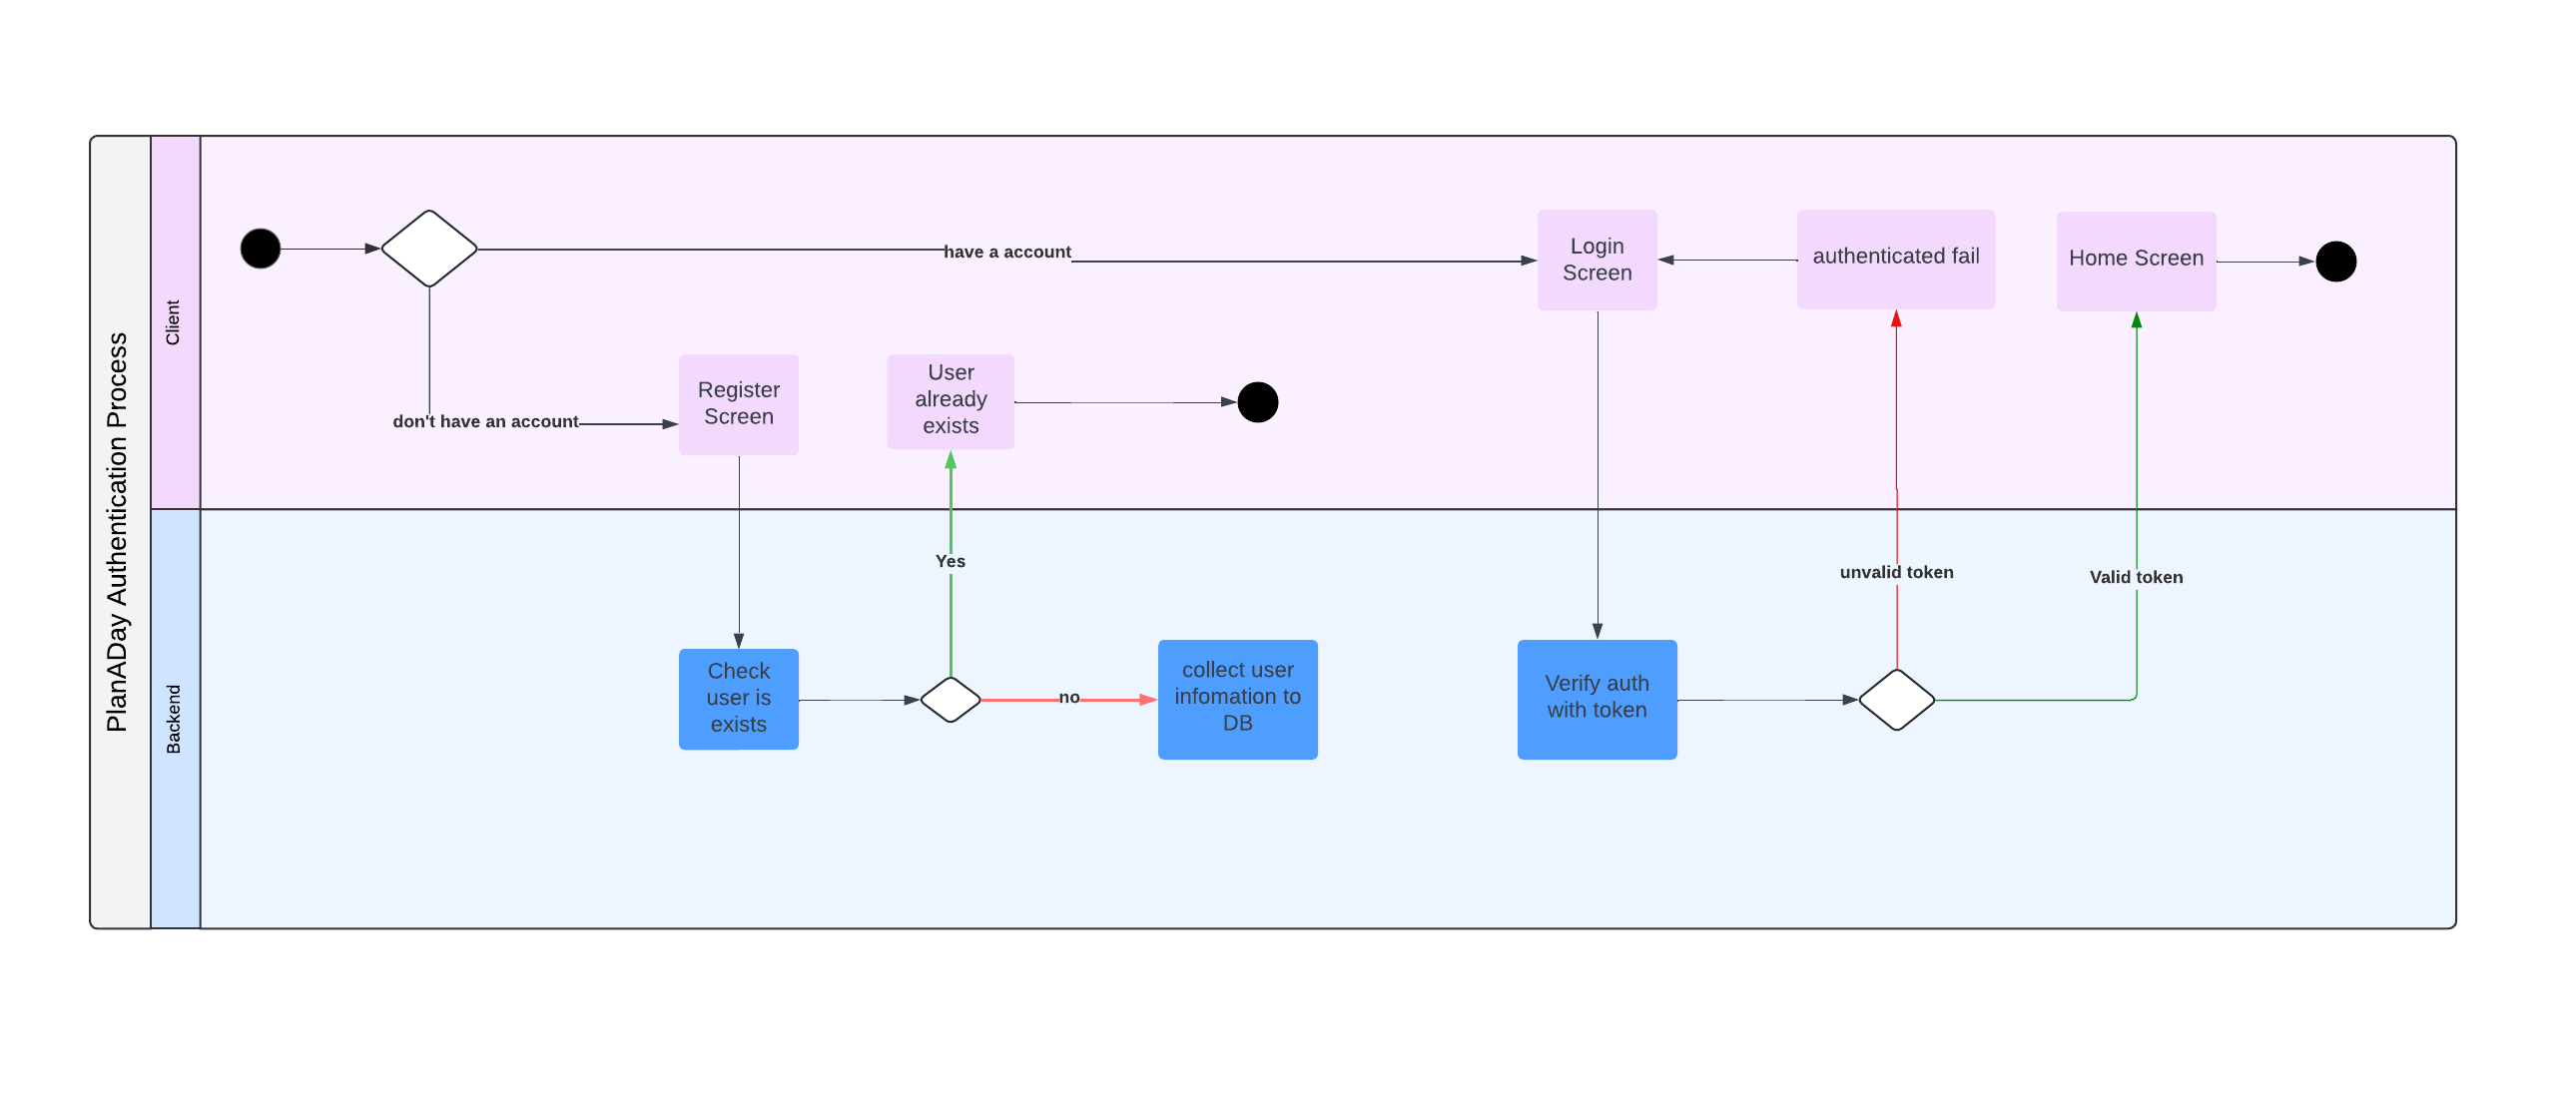
\includegraphics[width=1\linewidth]{chapter3/authentication-process.png}
    \caption{Activity Diagram of Authentication Process}
    \label{fig:Activity Diagram of Authentication Process}
\end{figure}
\par
The PlanADay Authentication Process illustrates the workflow for user registration and login,
divided into client-side and backend interactions. The process begins with a decision: if the user
does not have an account, they are directed to the registration screen. On registering, the backend
checks if the user already exists. If the user exists, they are informed and redirected to the login
screen; otherwise, their information is collected and stored in the database. For users with an
account, the login screen allows them to authenticate. The backend verifies the authentication
using a token. If the token is valid, the user is granted access to the home screen. In the event of
an invalid token, authentication fails. This flow ensures a secure and user-friendly mechanism
for handling account creation and login.
\newpage
Generate Plan Process
\begin{figure}[!h]
    \centering
    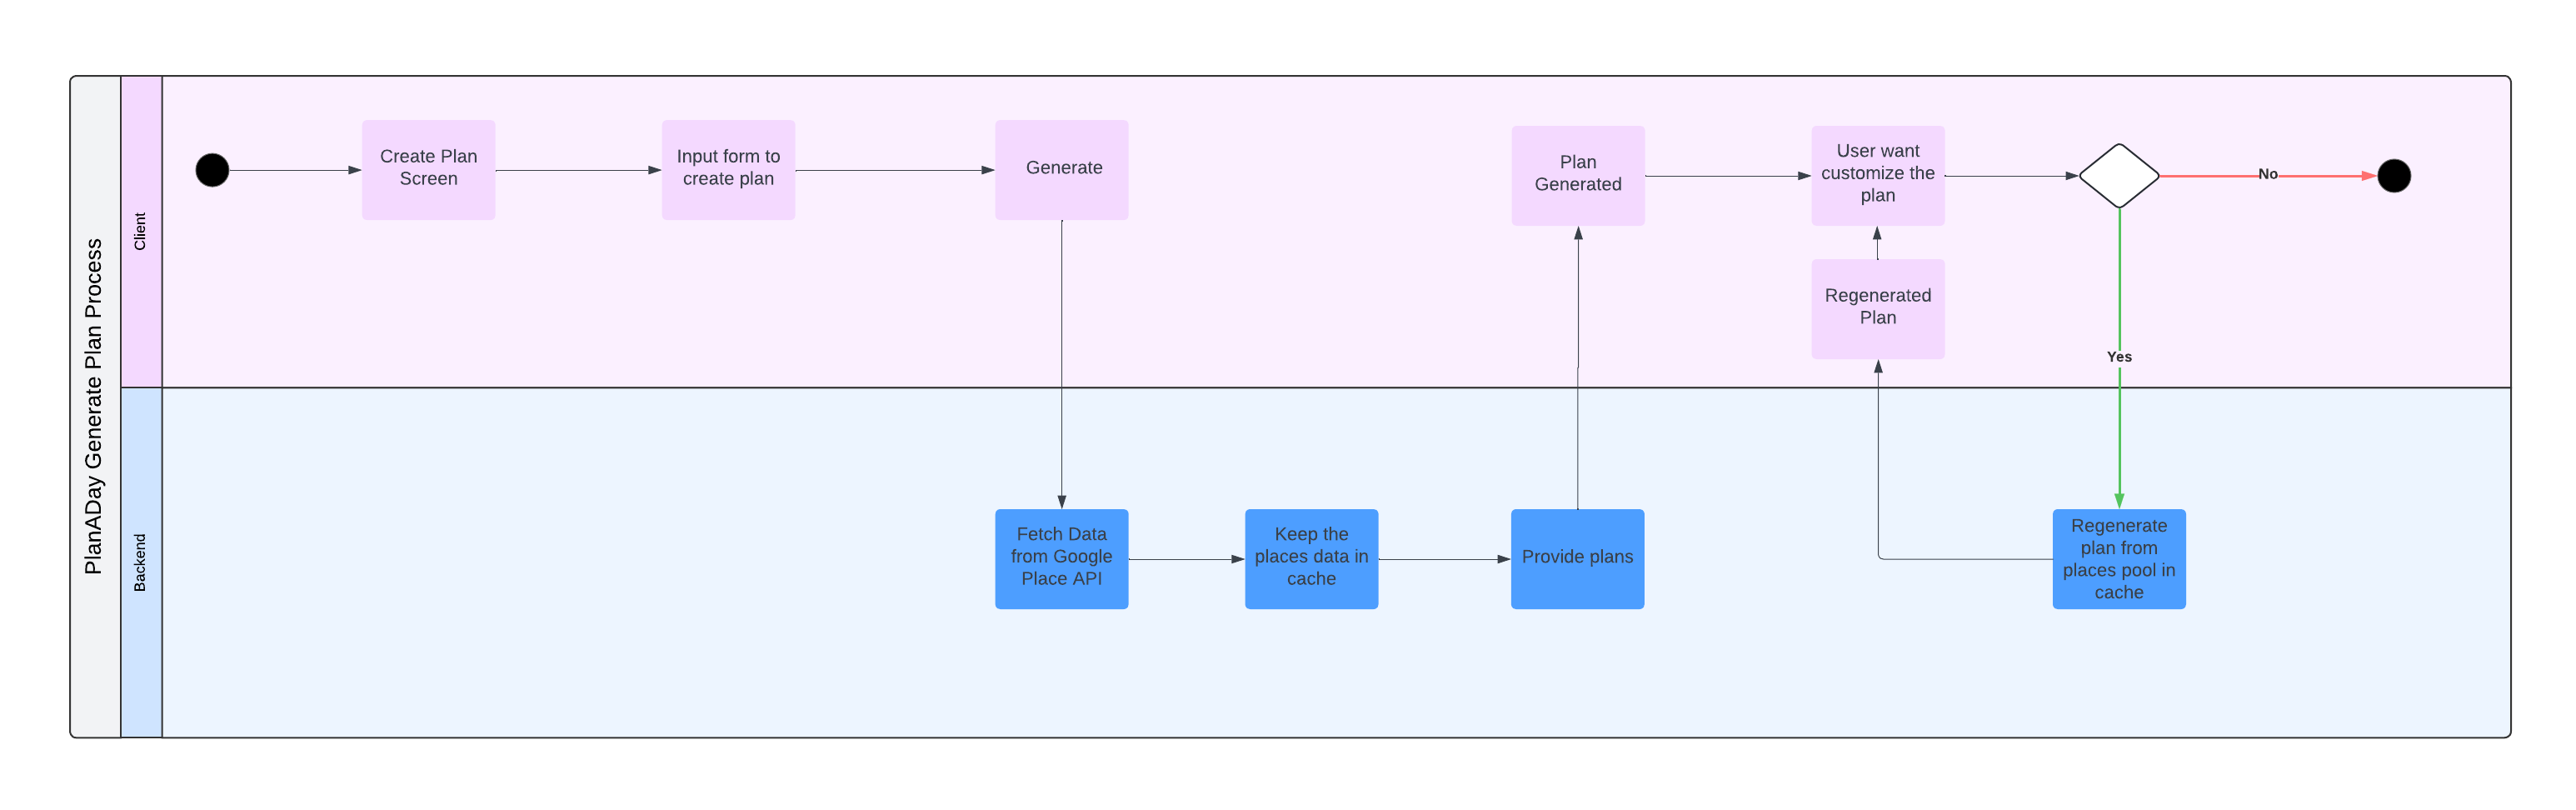
\includegraphics[width=1\linewidth]{chapter3/generate-process.png}
    \caption{Activity Diagram of Generate Plan Process}
    \label{fig:Activity Diagram of Generate Plan Process}
\end{figure}
\par
The PlanADay Generate Plan Process outlines the workflow for creating and customizing
plans. The process begins on the client side, where the user accesses the "Create Plan" screen,
fills out an input form, and initiates the plan generation. The backend fetches relevant data from
the Google Places API, caches the data for future use, and provides the generated plan to the
client. After the plan is displayed, the user has the option to customize it. If they choose to do so,
the backend regenerates the plan using the cached data without making additional API calls. If
no customization is needed, the process ends. This workflow ensures efficiency through caching
and provides a seamless user experience for generating personalized plans.
\newpage
\subsection{User Interface Design}

%Gift Handle this Plese !!!!!!!!!!!!!!!

\newpage
\section{Database design}
\subsection{Relational Database}
\begin{figure}[!h]
	\centering
	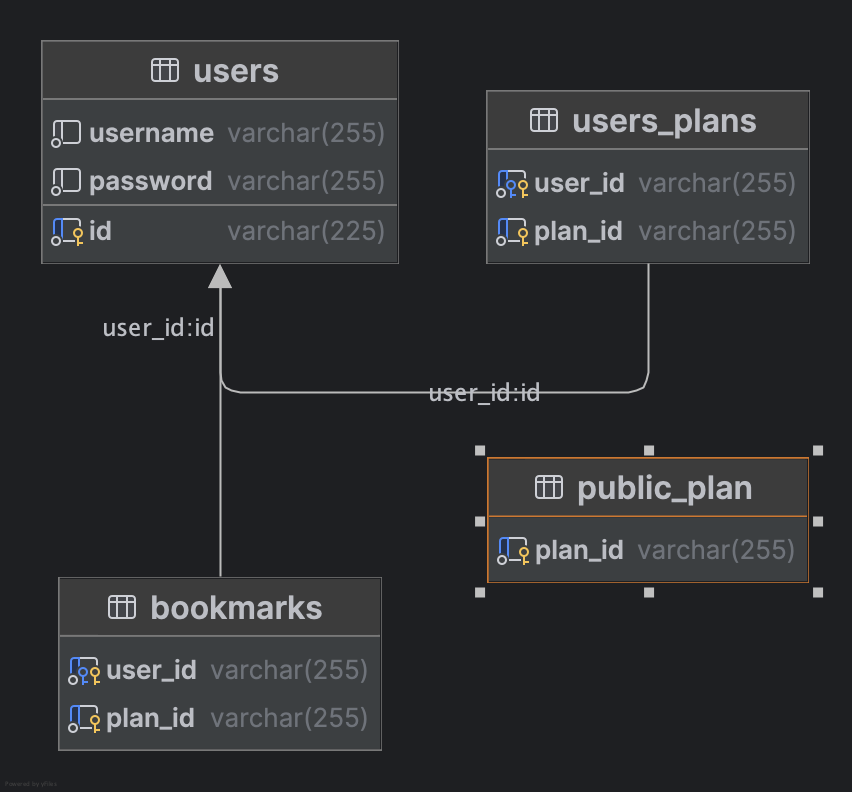
\includegraphics[width=0.5\linewidth]{chapter3/relational-database.png}
	\caption{Relational Database Schema}
	\label{fig:Relational Database Schema}
\end{figure}
Our database relies on PostgreSQL. The ER diagram illustrates a system for managing public
plans and user interactions with them. Public plans are stored in the public-plan entity, identified
by their unique plan-id. Users are represented in the users entity with their username, password,
and id. The users-plans entity establishes a many-to-many relationship between users and public
plans, allowing users to be associated with multiple plans and vice versa. The bookmarks entity
also represents a many-to-many relationship, enabling users to bookmark multiple public plans
and plans to be bookmarked by multiple users.
\newpage
\subsection{non-relational database}
\begin{figure}[!h]
    \centering
    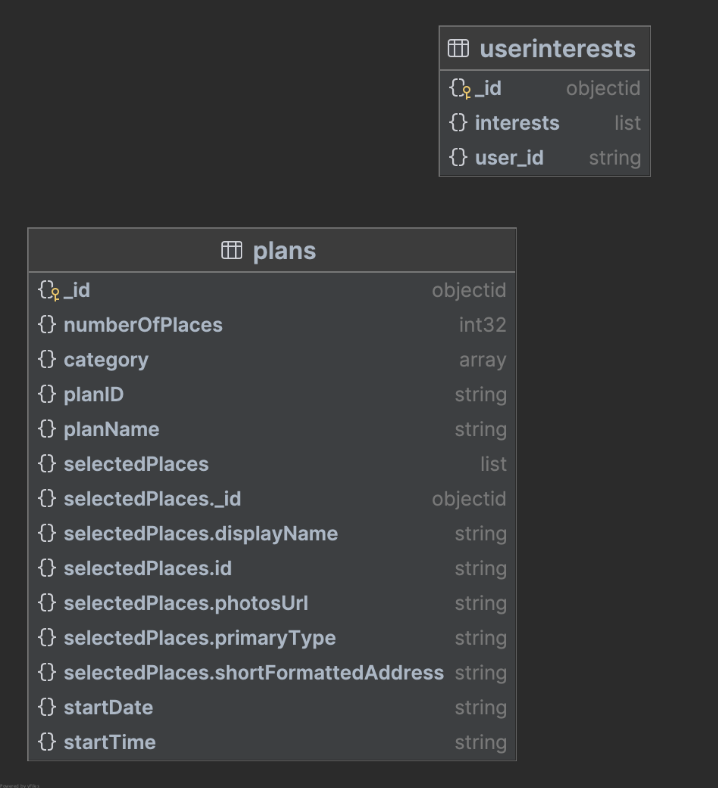
\includegraphics[width=0.6\linewidth]{chapter3/no-sql-diagram.png}
    \caption{Non-Relational Database Schema}
    \label{fig:Non-Relational Database Schema}
\end{figure}
The ER diagram depicts a database schema for managing travel plans and user interests. The
user interests table stores user IDs and their associated interests. The plans table contains detailed
information about travel plans, including the number of places, category, plan ID, name, selected
places with their attributes, and start date/time.